%------------------------------------------------------------------------
%Editar Diplomado
\hypertarget{cv:GestionarPExt}{\section{Gestionar Puntos de Extensión}} \label{sec:GestionarPExt}

	Esta funcionalidad le permitirá las acciones necesarias para controlar los puntos de extensión de un caso de uso y visualizarlos en una tabla en el proyecto sobre el que se está operando y solicitar el registro de uno nuevo.

		\subsection{Procedimiento}

			%Pasos de procedimiento
			\begin{enumerate}
			
			\item Oprima el botón \IUPext{} de algún registro existente de la pantalla \ref{fig:GestionarCU} ''Gestionar Casos de Uso''.
	
			\item Se mostrará la pantalla \ref{fig:GestionarPuntosExt} ''Gestionar Puntos de Extensión''.

			%Pantalla
			\begin{figure}[htbp!]
				\begin{center}
					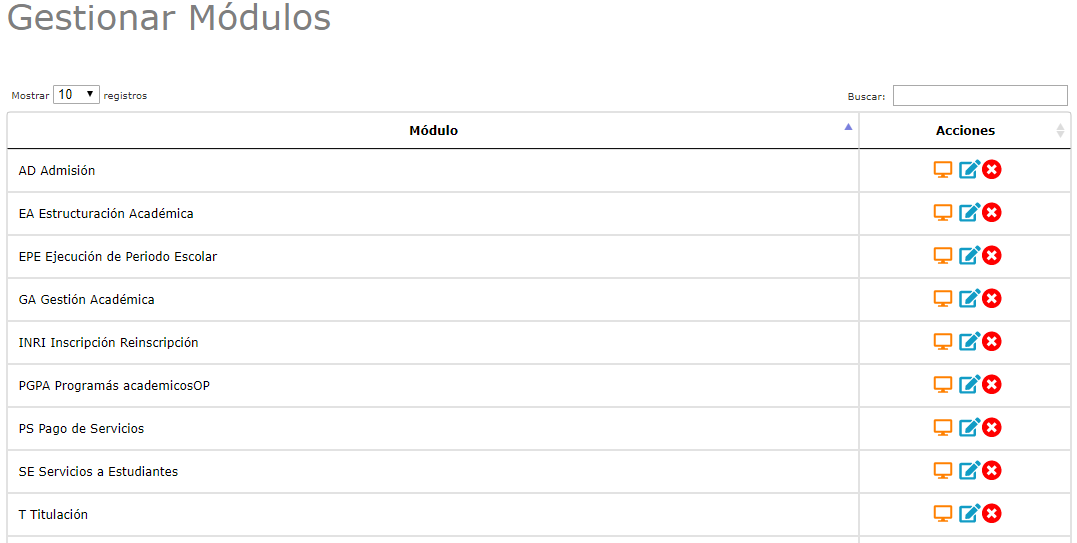
\includegraphics[scale=0.6]{roles/lider/casosUso/pantallas/IU5gestionarModulos}
					\caption{Gestionar Puntos de Extensión}
					\label{fig:GestionarPuntosExt}
				\end{center}
			\end{figure}
		
				\item Seleccione la operación que desea realizar:
			
			Para (\hyperlink{cv:registrarPExt}{Registrar}) dé clic en el botón \IURegistrar.
			
			Para (\hyperlink{cv:modificarPExt}{Modificar}) dé clic en el icono \IUEditar{} de algún punto de extensión ya registrado.
			
			Para (\hyperlink{cv:eliminarPExt}{Eliminar}) dé clic en el icono \IUBotonEliminar{} de algún punto de extensión ya registrado.
			
			\end{enumerate}